\chapter{Design and Implementation}
\label{chap:design_and_implementation}

In this chapter, we will discuss the design and implementation of the \ac{POP} algorithm.
We will start by discussing the design of the algorithm,
and then we will discuss the implementation of the algorithm in C\#.

\section{Design of the System}
In this section, we will discuss the design of the system, including the design of the \ac{POP} algorithm, and the design of Unity components that were used to visualize the \ac{POP} algorithm.
\subsection[POP Algorithm]{\ac{POP} Algorithm} \label{subsec:pop_algorithm_design}

This section will discuss some of the design decisions that were made during the implementation of the \ac{POP} algorithm. It will include an overview of the implemented algorithms that were used beside the \ac{POP} algorithm. In addition, it will discuss the data structures that were used to represent the planning domain and the planning problem.

\subsubsection{Nondeterministic Achievers \& Threat Search} \label {subsubsec:nondeterministic_achievers_threat_search}
\acf{POP} needs to be able to handle some form of nondeterminism in the planning domain. This is because the planner needs
to be able to handle situations where there are multiple ways to achieve a precondition
of an action. Nondeterminism is a concept that is used in computer science to describe the occurrence of events without a predictable outcome, where multiple outcomes are possible from a given state. In the context of planning, nondeterminism is used to describe the situation where there are multiple ways to achieve a precondition of an action, for example.
This cannot be achieved in practice without trying to search all possible ways of the choices that can be made.
So, to model nondeterminism in the planning domain, we need to use some form of graph search algorithm to search for all possible ways to achieve a precondition of an action efficiently. In this project, multiple graph search algorithms were implemented to handle nondeterminism in the planning domain. These algorithms are \ac{A*} Search, \ac{BFS}, and \ac{DLS} which is a variation of \ac{DFS}. All of these algorithms are discussed in detail in the following sections.


\subsubsection{Graph Search Algorithms} \label{subsec:graph_search_algorithms}
Graph search algorithms are widely used in computer science to solve problems that can be represented as graphs. They have many applications in various fields such as artificial intelligence, computer graphics, and computer vision. In this project, graph search algorithms were used to solve the problem of nondeterminism in the planning domain.
The following graph search algorithms were implemented in the project:
\begin{itemize}

    \item \textbf{\acf{A*} Search Algorithm} \label{subsubsec:a_star} \\
          \ac{A*} Search is a graph search \& traversal algorithm that is widely used in computer science due to its efficiency, optimality, and completeness. It is an informed search algorithm that uses a heuristic function to estimate the cost of reaching the goal from a given state. The heuristic function is used to guide the search towards the goal state by selecting the most promising nodes to explore. \ac{A*} Search is an extension of Dijkstra's algorithm that uses a heuristic function to estimate the cost of reaching the goal from a given state. \ac{A*} is a Best First Search algorithm that uses a priority queue to store the nodes to be explored. The priority queue is ordered based on a cost function that combines the cost of reaching the node from the start state and the heuristic estimate of the cost of reaching the goal from the node. The cost function is defined as $f(n) = g(n) + h(n)$, where $g(n)$ is the cost of reaching the node from the start state and $h(n)$ is the heuristic estimate of the cost of reaching the goal from the node. The algorithm selects the node with the lowest $f$ value from the priority queue and explores its neighbors until the goal is reached. The algorithm is guaranteed to find the optimal solution if the heuristic function is admissible, i.e., it never overestimates the cost of reaching the goal from a given state. The algorithm is also complete if the search space is finite and the heuristic function is consistent.

          In this project, $g(n)$ is the path (level) cost from the root node to the current node, and $h(n)$ heuristic was chosen to be the number of unsatisfied preconditions, i.e., the count of pairs in the $agenda$ discussed in section {\ref{subsec:pop_algorithm}}.

    \item \textbf{\acf{DLS} Search Algorithm} \label{subsubsec:dls}\\
          First, let's discuss the \ac{DFS} algorithm.
          \ac{DFS} is an uninformed search algorithm that is widely used in computer science to explore a graph or tree data structure. It is a depth-first traversal algorithm that explores the nodes deep in the graph before exploring the nodes at the same level. The algorithm starts at the root node and explores the nodes along each branch before backtracking to explore the other branches. The algorithm uses a stack data structure to store the nodes to be explored. The algorithm is not guaranteed to find the optimal solution, but it is complete if the search space is finite. The algorithm is also efficient in terms of memory usage as it only needs to store the nodes along the current path. However, the algorithm can get stuck in infinite loops if the graph contains an infinite deep path. To avoid this problem, a depth limit can be imposed on the search to limit the depth of the search tree. This is known as the \acf{DLS} algorithm. The algorithm is similar to \ac{DFS} but with an additional depth limit parameter that specifies the maximum depth of the search tree. The algorithm stops exploring a branch when the depth limit is reached and backtracks to explore other branches. The algorithm is complete if the depth limit is greater than the depth of the optimal solution. The algorithm is also efficient in terms of memory usage. In this project, \ac{DLS} was also provided as an option to be used in the \ac{POP} algorithm.

    \item \textbf{\acf{BFS} Search Algorithm} \label{subsubsec:bfs}\\
          \ac{BFS} is an uninformed search algorithm that is widely used to explore a graph or tree data structure. It is a breadth-first traversal algorithm, meaning that it explores the nodes at the same level before exploring the nodes at the next level. The algorithm starts at the root node and explores the nodes at the same level before moving to the next level. The algorithm uses a queue data structure to store the nodes to be explored. The algorithm is guaranteed to find a solution if one exist, even if the graph is infinite. However, the algorithm is not guaranteed to always find the optimal solution. The algorithm is also inefficient in terms of memory usage as it needs to store all the nodes at the current level. In this project, \ac{BFS} was also provided as an option to be used in the \ac{POP} algorithm.

          \subsubsection{Unification Algorithm} \label{subsubsec:unification_algorithm}
          Finding the \acf{MGU} of two terms is a crucial step in the \ac{POP} algorithm. The \ac{MGU} is used to unify two terms by finding a substitution that makes the two terms equal. The \ac{MGU} is the most general substitution that can be applied to the two terms to make them equal.
          For example, consider the following terms: $P(x, B)$ and $P(A, y)$. The \ac{MGU} of these two terms is $\{x/A, y/B\}$, which means that the terms can be unified by substituting $A$ for $x$ and $B$ for $y$ to make them equal to $P(A, B)$.
          The \ac{MGU} is used to unify the preconditions of an action with the current state of the world to determine if the action can be applied. The \ac{MGU} is also used to unify the effects of an action that can be used, for example, to detect threats in the partial plan.
          In this project, the \ac{MGU} algorithm was implemented using a variation of the unification algorithm discussed in Russell and Norvig's book \cite{RN2020_Ch.9}, and taken from the lecture slides of the course \textit{Introduction to Artificial Intelligence} by Prof. Haythem Ismail \cite{Ismail2023}.
          The algorithm described in \autoref{alg:unification_algorithm} has three main functions: UNIFY, UNIFY1, and UNIFYVAR. The UNIFY function takes two exrpressions as input, listifies them, and then calls the UNIFY1 function with the two listified expressions and an empty substitution set. An example of listifying an expression is converting the expression $P(x, f(y,z))$ to the list $[P, x, [f, y, z]]$. The UNIFY1 function takes two listified expressions and a substitution set as input and returns the most general unifier of the two expressions. The UNIFYVAR function takes a variable, an expression, and a substitution set as input and returns the most general unifier of the variable and the expression. The main algorithm starts in line 6 by checking if the substitution set is a failure, in which it returns a failure. Then, it checks if the two expressions are equal, in which it returns the curernt substitution set. Then, it checks if $E1$ or $E2$ is a variable, in which it calls the UNIFYVAR function with the first parameter being the variable and the second parameter being the expression. Then, it checks if $E1$ or $E2$ is an atom, in which it returns a failure in line 19. The reason for this is that after making sure that neither $E1$ or $E2$ are variables, and they are not equal, then they must be different atoms, and thus cannot be unified. Then, it checks if the length of $E1$ is not equal to the length of $E2$, in which it returns a failure in line 22, as we cannot unify two expressions with different lengths, like $P(x)$ and $P(x, y)$. Finally, it calls the UNIFY1 function recursively with the rest of the two expressions and the unification of the first elements of the two expressions. The UNIFYVAR function starts by checking if the variable $x$ is already in the substitution set and bound to a term $t$ that is not equal to $x$, in which it calls the UNIFY1 function with the term $t$ and the input expression $e$. If the variable $x$ is not in the substitution set, then it substitutes every term in the expression $e$ with the substitution set $\mu$. Then, it checks if the variable $x$ occurs in the term $t$, in which it returns a failure, as we cannot unify a variable with an expression that contains the variable. If we had $x$ and $f(x)$, then the unification would fail, since it would result in an infinite recursion.
          Otherwise, it returns the substitution set $\mu$ composite with the substitution $\{t/x\}$, which means that the term $t$ is substituted for the variable $x$ in the substitution set $\mu$.

          \begin{algorithm}
              \caption{Unification Algorithm}
              \begin{algorithmic}[1]
                  \label{alg:unification_algorithm}
                  \STATE \textbf{function} UNIFY($E1, E2$) :
                  \RETURN UNIFY1(LISTIFY($E1$), LISTIFY($E2$), $\{\}$);
                  \STATE
                  --------------------------------------------------------------------------------------------------------
                  \STATE
                  \STATE \textbf{function} UNIFY1($E1, E2, \mu$) :
                  \IF{$\mu = \text{fail}$}
                  \RETURN fail
                  \ENDIF
                  \IF{$E1 = E2$}
                  \RETURN $\mu$
                  \ENDIF
                  \IF{VAR?($E1$)}
                  \RETURN UNIFYVAR($E1, E2, \mu$)\ENDIF
                  \IF{VAR?($E2$)}
                  \RETURN UNIFYVAR($E2, E1, \mu$)
                  \ENDIF
                  \IF{ATOM?($E1$) or ATOM?($E2$)}
                  \RETURN fail
                  \ENDIF
                  \IF{LENGTH($E1$) != LENGTH($E2$)}
                  \RETURN fail
                  \ENDIF
                  \RETURN UNIFY1(REST($E1$), REST($E2$), UNIFY1(FIRST($E1$), FIRST($E2$), $\mu$))
                  \STATE
                  --------------------------------------------------------------------------------------------------------
                  \STATE
                  \STATE \textbf{function} UNIFYVAR($x, e, \mu$) :
                  \IF{$t/x \in \mu$ and $t \neq x$}
                  \RETURN UNIFY1($t, e, \mu$)
                  \ENDIF
                  \STATE $t = \text{SUBST}(\mu, e)$
                  \IF{$x$ occurs in $t$}
                  \RETURN fail
                  \ELSE
                  \RETURN $\mu \circ \{t/x\}$
                  \ENDIF
              \end{algorithmic}
          \end{algorithm}

\end{itemize}


% image of the pop class diagram (POP.png)
\begin{figure}[ht]
    \centering
    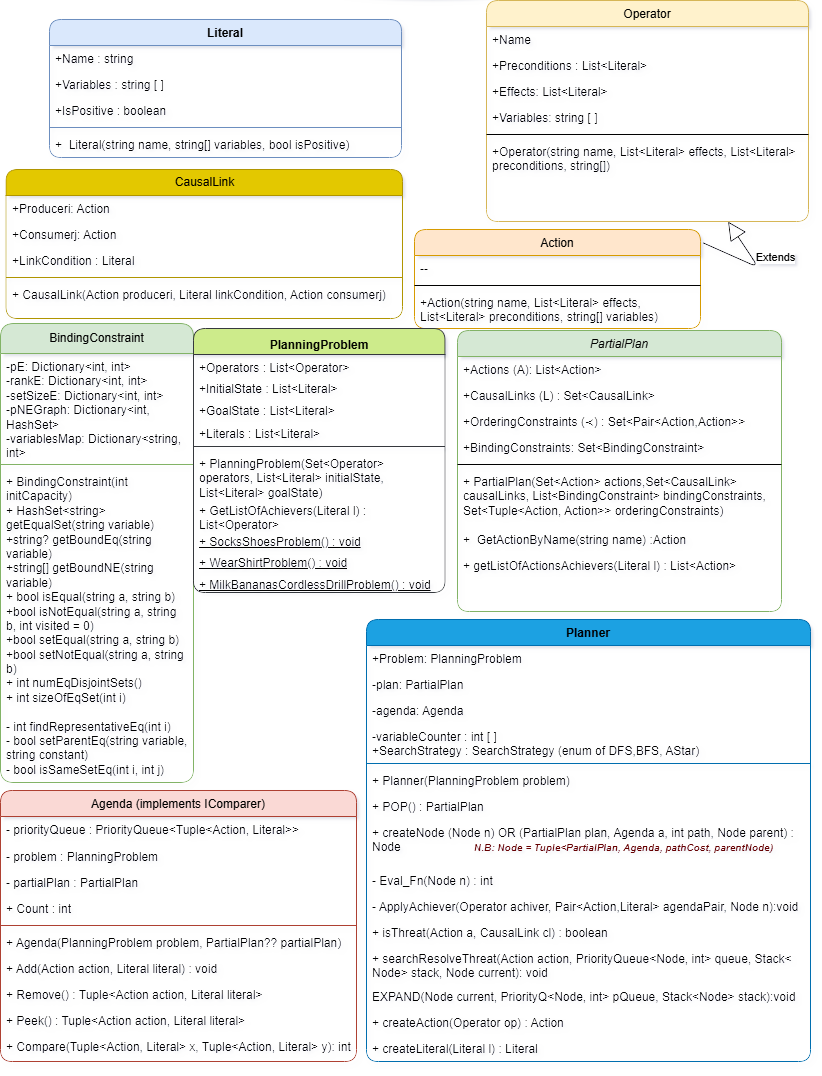
\includegraphics[width=0.9\textwidth]{images/POP.png}
    \caption[Class Diagram of the POP Algorithm]{Class Diagram of the POP Algorithm}
    \label{fig:pop}
\end{figure}
